\subsection{GSM (2G)}
\selectlanguage{russian}

Регистрация телефона в сети GSM построена с участием трёх сторон: SIM-карты мобильного устройства, базовой станции и центра аутентификации. SIM-карта и центр аутентификации обладают общим секретным 128-битным ключом $K_i$. Вначале телефон сообщает базовой станции уникальный идентификатор SIM-карты IMSI открытым текстом. Базовая станция запрашивает в центре аутентификации для данного IMSI набор параметров для аутентификации. Центр генерирует псевдослучайное 128-битовое число $\textrm{RAND}$ и алгоритмами A3\index{алгоритм!A3} и A8\index{алгоритм!A8} создаёт симметричный 54-битовый ключ $K_c$ и 32-битовый аутентификатор $\textrm{RES}$. Базовая станция передаёт мобильному устройству число $\textrm{RAND}$ и ожидает результата вычисления SIM-картой числа $\textrm{XRES}$, которое должно совпадать с $\textrm{RES}$ в случае успешной аутентификации. Схема аутентификации показана на рис.~\ref{fig:gsm2}.

\begin{figure}[!ht]
	\centering
	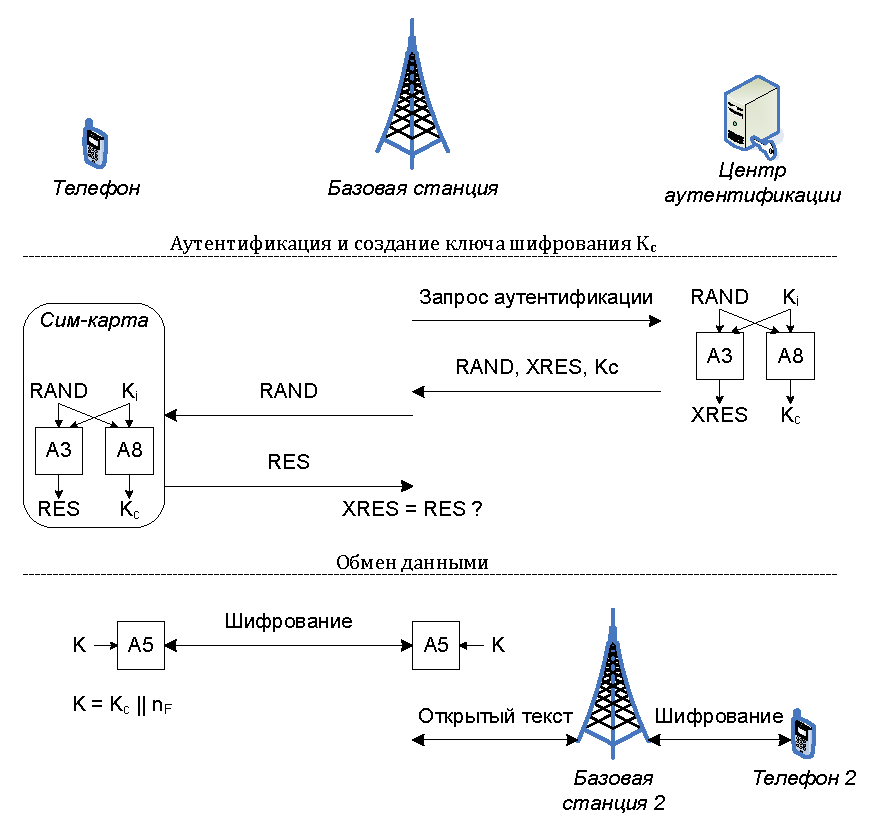
\includegraphics[width=0.85\textwidth]{pic/gsm2}
	\caption{Односторонняя аутентификация и шифрование в GSM\label{fig:gsm2}}
\end{figure}

Все вычисления для аутентификации выполняет SIM-карта. Ключ $K_c$ далее используется для создания ключа шифрования каждого фрейма $K = K_c ~\|~ n_F$, где $n_F$~--~22-битовый номер фрейма. Шифрование выполняет уже само мобильное устройство. Алгоритм шифрования фиксирован в каждой стране и выбирается из семейства алгоритмов A5\index{шифр!A5} (A5/1, A5/2, A5/3). В GSM применяется либо шифр A5/1 (используется в России), либо A5/2. Шифр A5/3 применяется уже в сети UMTS.

Аутентификация в сети GSM односторонняя. При передаче данных не используются проверка целостности и аутентификация сообщений. Передача данных между базовыми станциями происходит в открытом незашифрованном виде. Алгоритмы шифрования A5/1 и A5/2 не стойкие, количество операций для взлома A5/1~--~$2^{40}$, A5/2~--~$2^{16}$. Кроме того, длина ключа $K_c$ всего 54 бита. Передача в открытом виде уникального идентификатора IMSI позволяет однозначно определить абонента.
